\let\negmedspace\undefined
\let\negthickspace\undefined
\documentclass[journal]{IEEEtran}
\usepackage[a5paper, margin=10mm, onecolumn]{geometry}
\usepackage{lmodern} % Ensure lmodern is loaded for pdflatex
\usepackage{tfrupee} % Include tfrupee package

\setlength{\headheight}{1cm} % Set the height of the header box
\setlength{\headsep}{0mm}     % Set the distance between the header box and the top of the text

\usepackage{gvv-book}
\usepackage{gvv}
\usepackage{cite}
\usepackage{amsmath,amssymb,amsfonts,amsthm}
\usepackage{algorithmic}
\usepackage{graphicx}
\usepackage{textcomp}
\usepackage{xcolor}
\usepackage{txfonts}
\usepackage{listings}
\usepackage{enumitem}
\usepackage{mathtools}
\usepackage{gensymb}
\usepackage{comment}
\usepackage[breaklinks=true]{hyperref}
\usepackage{tkz-euclide} 
\usepackage{listings}
\usepackage{gvv}                                        
\def\inputGnumericTable{}                                 
\usepackage[latin1]{inputenc}                                
\usepackage{color}                                            
\usepackage{array}                                            
\usepackage{longtable}                                       
\usepackage{calc}                                             
\usepackage{multirow}                                         
\usepackage{hhline}                                           
\usepackage{ifthen}                                           
\usepackage{lscape}
\begin{document}

\bibliographystyle{IEEEtran}
\vspace{3cm}

\title{9.1.8}
\author{EE24BTECH11005 - Arjun Pavanje}
% \maketitle
% \newpage
% \bigskip
{\let\newpage\relax\maketitle}
\textbf{Question:}
Solve the differential equation $y^{\prime}+y=e^x$ with initial conditions $y\brak{0}=1$
\solution\\

\textbf{Theoretical Solution}\newline
Given equation is a linear first order differential equation, so laplace transform may be used to solve it. Some properties of laplace transform used are,
\begin{align}
  \mathcal{L}\brak{f\brak{t}} &= \int_0^{\infty} e^{-st} f\brak{t} \, dt\\
 \mathcal{L}\brak{\kappa f\brak{t}} &= \kappa \mathcal{L}\brak{f\brak{t}}\\
  \mathcal{L}\brak{y^{\prime}} &= sY\brak{S} - y_0
\end{align}
Where $\mathcal{L}\brak{y} = Y\brak{s}$
Applying Laplace Transform to given differential Equation,
\begin{align}
  \mathcal{L}\brak{y^{\prime}} + \mathcal{L}\brak{y} &= \mathcal{L}\brak{e^{x}}\\
  sY\brak{s} - y_0 + Y\brak{S} &= \int_0^{\infty} e^{-x\brak{x - 1} } dx = \frac{1}{s-1}\\
  Y\brak{s} &= \brak{\frac{y_0 - 0.5}{s+1}} + \frac{1}{2}\brak{\frac{1}{s-1}}
 \end{align}
 Taking Laplace Inverse on both sides we get,
 \begin{align}
   y &= \mathcal{L}^{-1}\brak{\frac{y_0 - 0.5}{s+1}} + \mathcal{L}^{-1}\frac{1}{2}\brak{\frac{1}{s-1}}\\
   y &= \brak{y_0 - 0.5}e^{-x} + \frac{1}{2} e^{x}
 \end{align}
 Putting in $y_0 = 1$ we get,
 \begin{align}
   y = \frac{\brak{e^{x} + e^{-x}}}{2}
 \end{align}\textbf{Computational Solution:}\newline
 Solving given differential equation using bilinear transform.
Taking Laplace transform to both sides of the Differential Equation,

\begin{align}
  sY\brak{s} - y_0 + Y\brak{s} = \int_0^{\infty} e^{-x\brak{x - 1} } dx = \frac{1}{s-1}\\
  Y\brak{s} = \frac{y_0}{s+1} + \frac{1}{\brak{s + 1} \brak{s - 1}}\\
  Y\brak{s} = \brak{\frac{y_0 - 0.5}{s+1}} + \frac{1}{2}\brak{\frac{1}{s-1}}
\end{align}

Applying Bilinear Transform with $T=h$. To go from the domain of Laplace transform to that of Z-transform, we transform our $s$. On substituting we get,

\begin{align}
  Y\brak{s} &= \brak{y_0 - 0.5}\brak{\frac{h\brak{1 + z^{-1}} }{ 2\brak{1 - z^{-1}} + h\brak{1 + z^{-1}} }} + \frac{1}{2}\brak{\frac{h\brak{1 + z^{-1}} }{ 2\brak{1 - z^{-1}} - h\brak{1 + z^{-1}} }}\\
  & = \brak{y_0 - 0.5}\brak{\frac{h\brak{1 + z^{-1}} }{ \brak{2+h} + z^{-1}\brak{h-2} } } +\frac{1}{2}\brak{\frac{h\brak{1 + z^{-1}} }{ \brak{2-h} + z^{-1}\brak{2+h} } }\\
  &= \brak{\frac{y_0 - 0.5}{2+h}} \brak{\frac{h\brak{1 + z^{-1}}}{1 - \alpha z^{-1}} } + \brak{\frac{h}{2\brak{2-h}}}\brak{\frac{h\brak{1+z^{-1}}}{1 - \alpha^{-1}z^{-1}}}
\end{align}
Where $\alpha = \frac{2-h}{2+h}$ \newline
Radius of convergence of the first term is, $\abs{z} > \abs{\alpha}$, for the second term it is, $\abs{z} > \abs{\alpha^{-1}}$. R.O.C of the total equation turns out to be, $\abs{z} > max \brak{\abs{\alpha}, \abs{\frac{1}{\alpha}}}$\newline
Taking $\brak{1 - \alpha z^{-1]}}$ to $R.H.S$ we get,
\begin{align}
  Y\brak{s}\brak{1 - \alpha z^{-1}} = h\brak{\frac{y_0 - 0.5}{2+h}}\brak{\brak{1 + z^{-1}} } + \brak{\frac{h}{2\brak{2-h}}}\brak{\frac{h\brak{1+z^{-1}} \brak{1 - \alpha z^{-1}} }{1 - \alpha^{-1}z^{-1}}}
\end{align}
After applying algebraic manipulations on the second term, above equation comes out to be, 
\begin{align}
  Y\brak{s}\brak{1 - \alpha z^{-1}} &= h\brak{ \frac{y_0 - 0.5}{2+h}}\brak{\brak{1 + z^{-1}} } + \\
  &\brak{\frac{h}{2\brak{2+h}}} \brak{ \frac{1 + \alpha - \alpha^2 - \alpha^3}{1 - \alpha^{-1}z^{-1}} + \alpha^2 z^{-1} - \alpha \brak{1 - \alpha - \alpha^2} } 
\end{align}
Applying inverse Z-transform,
\begin{align}
  y_{n+1} &= \alpha y_n + h\brak{ \frac{y_0 - 0.5}{2+h}}\brak{\delta \sbrak{n} + \delta \sbrak{n-1}}+ \brak{\frac{h}{2\brak{2+h}}} \times \\
  &\brak{\brak{1 + \alpha - \alpha^2 - \alpha^3}\alpha^{-n} u \brak{n} + \alpha^2 \delta \sbrak{n-1}- \alpha \brak{1 - \alpha - \alpha^2} \delta \sbrak{n} }
\end{align}
here, $\delta$ is defined as,
\begin{align}
  \delta \sbrak{n-n_0} = \begin{cases}
      1 & n = n_0 \\
      0 & n \ne n_0
  \end{cases}
\end{align}
Final General Difference Equation comes out to be, 
\begin{align}
  y_{n+1} &= \alpha y_n + h\brak{ \frac{y_0 - 0.5}{2+h}}\brak{\delta \sbrak{n} + \delta \sbrak{n-1}}+ \brak{\frac{h}{2\brak{2+h}}} \times \\
  &\brak{\brak{1 + \alpha - \alpha^2 - \alpha^3}\alpha^{-n} u \brak{n} + \alpha^2 \delta \sbrak{n-1}- \alpha \brak{1 - \alpha - \alpha^2} \delta \sbrak{n} }
\end{align}

\textbf{Alternate Computational Solution}\newline

Finding the difference equation using trapezoid law,

Given Differential Equation,
\begin{align}
  y^{\prime} &= -y + e^x \\
  \int_{y_n}^{y_{n+1}} dy &= -\int_{x_n}^{x_{n+1}} ydx +\int_{x_n}^{x_{n+1}} e^x dx  
\end{align}
Discretizing steps using trapezoid rule, 
\begin{align}
  y_{n+1} = y_n - \frac{h}{2}\brak{y_n + y_{n+1}} + e^{x_n}(e^h-1)
\end{align}
\begin{align}
  y_{n+1} - y_n &= -\frac{h}{2}\brak{y_n + y_{n+1}} + e^{x_n}\brak{e^h-1}\\
  y_{n+1} &= y_n\brak{\frac{2-h}{2+h}} + \frac{2e^{x_n}}{2+h}\brak{e^h-1}
\end{align}
\begin{figure}[h!]
   \centering
   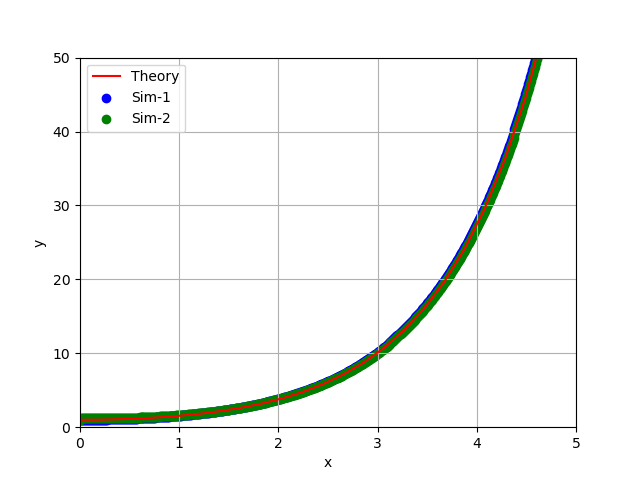
\includegraphics[width=1\columnwidth]{figs/fig.png}
   \caption{Differential Equation $y^{\prime}+y=e^x$ solved using Bilinear transform. Sim-1 shows plot obtained by using trapezoidal law, Sim-2 shows plot obtained by using Bilinear transform method. Theory shows plot obtained theoretically}
   \label{stemplot}
\end{figure}
\end{document}
